
%----------------------
%	CHAPTER 1
%----------------------

\chapterimage{chapter_head_2.pdf} % Chapter heading image

\chapter{\texorpdfstring{Relations, Mappings, and $\Z$}{Relations, Mappings, and Z (integers)}}
\vspace{-0.25 in}
\section{Relations and Equivalence Relations}
We begin with a discussion of relations, equivalence relations, and equivalence classes. This section concludes with a fundamental correspondence between equivalence relations and partitions of sets.
\begin{definition}[Relations]
A \textit{relation}\footnote{
    A relation \textit{between} sets $A$ and $B$ is a subset $R\subset A\times B$ with $(a,b)\in R \iff a\sim b $. If $A=B$ the relation is called ``homogeneous" and we commonly say relation ``on" $A$ as above, if $A\neq B$ the relation is called ``heterogeneous"
} on a set $A$ is a statement in two variables which is either true or false for values in $A$
\end{definition}
\begin{example}
\label{ex:firstExample}
$A=\{\text{people in this room}\}$\\
$x\sim y \Leftrightarrow x \text{ was born in the same month as } y$\\
Read the above expression as ``$x$ is related to $y$ if and only if (iff) $x$ was born in the same month as $y$"
\end{example}
\begin{example}
    \label{ex:secondExample}
$A=\mathbb{R}$\\
$x\sim y \Leftrightarrow x \geq y$\\
so if we think of $\sqrt{2}$ and $0$ we have that $\sqrt{2}\geq 0$ so $\sqrt{2}\sim 0$, \\
However, since $0 \not\geq \sqrt{2} \Rightarrow 0\not\sim \sqrt{2}$
\end{example}
\begin{definition}[Reflexive, Symmetric, and Transitive Relations]
The relation $\sim$ on a set $A$ is said to be:
\begin{enumerate}[label=\roman*)]
    \item \textit{Reflexive} iff $x\sim x \ \forall x \in A$
    \item \textit{Symmetric} iff $x\sim y \Rightarrow y\sim x \ \forall \ x,y \in A$
    \item \textit{Transitive} iff $x\sim y$ and $y\sim z \Rightarrow x\sim z \ \forall x,y,z \in A$
\end{enumerate}
\end{definition}
A relation need not have any of these properties but if \textit{all three} of these properties hold, then $\sim$ is an \textit{equivalence relation} but that's important enough to get its own definition:
\begin{definition}[Equivalence Relation]
A relation $\sim$ on a set $A$ is an \textit{equivalence relation} if all three of the following hold:
\begin{enumerate}[label=\roman*)]
    \item Relation $\sim$ on $A$ is reflexive.
    \item Relation $\sim$ on $A$ is symmetric.
    \item Relation $\sim$ on $A$ is transitive.
\end{enumerate}
\end{definition}
Note that Example \ref{ex:firstExample} is an equivalence relation, but Example \ref{ex:secondExample} is not because it is not symmetric.
\newpage
\begin{example}
The relation ``equals" (``=") is an equivalence relation on $\mathbb{R}, \mathbb{Q}, \mathbb{Z}$ (i.e. on reals, rationals and integers). In fact, an equivalence relation is a generalization of equality, measuring equality up to some property.
\end{example}
% \noindent\textbf{Example 3:} The relation ``equals" (``=") is an equivalence relation on $\mathbb{R}, \mathbb{Q}, \mathbb{Z}$ (i.e. on reals, rationals and integers) \steezybreak\\
\begin{definition}[Even]
$n\in \mathbb{Z}$ is \textit{even} iff $n$ is an integer multiple of $2$ \\
that is, \\
$n\in \mathbb{Z} \text{ is}\textit{ even }\Leftrightarrow \exists \ k \in \mathbb{Z}$ such that $n=2k$
\end{definition}
%\noindent\textbf{Defn:} $n\in \mathbb{Z}$ is ``even" iff $n$ is an integer multiple of $2$ \\
%$\Leftrightarrow \exists k \in \mathbb{Z}$ such that $n=2k$\steezybreak\\

\begin{example}
Prove that $\sim$ is an equivalence relation on $\mathbb{Z}$:\\
$x\sim y \iff x-y \text{ is even}$\steezybreak\\

\noindent\textbf{Proof:} To prove we must show $\sim$ is reflexive, symmetric, and transitive on $\mathbb{Z}$.\\
\textit{Reflexivity:} Take $x\in \mathbb{Z}$, then $x-x=0=2*0$, since $0\in \mathbb{Z}$, $x-x$ is even. $\implies x\sim x \ \forall x \in \mathbb{Z}$\\
\textit{Symmetry:} Assume $x\sim y$, then $x-y$ is even which means $\exists k \in \mathbb{Z}$ such that $x-y=2k$. From here we can see $y-x=-(x-y)=-2k=2(-k)$, since $k\in \mathbb{Z}$, $-k\in \mathbb{Z}$ so $y-x$ is even too so we have $y\sim x$\\
\textit{Transitivity:} Assume $x\sim y$ and $y \sim z$. These expression imply the existence of two integers. The first expression implies $\exists \ k\in \mathbb{Z}$ such that $x-y=2k$ and the second expression implies $\exists \ l \in \mathbb{Z}$ such that $y-z=2l$. Using these we can see that $x-z=x-y+y-z=2k+2l=2*(k+l)$ since $k+l$ is a sum of integers, it is itself an integer so $x-z$ is even which implies $x\sim z$. So we have shown that assuming $x\sim y \text{ and } y\sim z \implies x\sim z \ \forall x,y,z \in \mathbb{Z}$. $\ \ \ \blacksquare$
\end{example}
\subsection{Understanding the First Proof}
Since this was the first proof in the course material we would like to take a few paragraphs to unpack the reasoning in the proof above. \steezybreak\\
\noindent We are asked to show that the relation defined in example 1.1.4 ($x\sim y \iff x-y \text{ is even}$) on $\Z$ is an equivalence relation. To do this we are required to show the defined relation exhibits three properties: reflexivity, symmetry, transitivity. We started by showing $\sim$ on $\Z$ has the reflexivity property. If we re-read the definition of reflexivity we see this property is a statement that pertains to \textit{every} element $a\in A$ for a relation that is defined on set $A$ (in this example $A=\Z$), it says that $\sim$ is reflexive on $A$ iff it is true that $a$ is related to itself for all $a\in A$. The reader may now be re-reading the proof and asking themselves ``So to prove $\sim$ is reflexive on $A$, don't we have to prove the reflexive property (i.e. $a\sim a$) holds for \textit{all} of the $a's$ in $A$? It looks like we only considered one?" This brings us to a very important point! \steezybreak\\

\noindent The first of these questions is certainly valid, and yes, we \textit{do} need to show this property holds for \textit{all} of the $x\in \Z$. However, the second question is a little misleading. We did consider a single $x\in \Z$, but this $x$ was \textit{arbitrary}, we did not pick $1$, or $2$ or $-664$, we instead chose "$x$", a \textit{variable}, to represent an arbitrary member of the set $\Z$ and then we \underline{only} made statements and inferences about $x$ that are true for \textbf{every} member of $\Z$ (i.e. we never used special properties of a specific member who $x$ could have been, such as $1$ or $2$, all we knew about $x$ is that it is an integer, and by being an integer it inherited any properties that are true for all integers). As a result, statements and inferences that were made about $x$ apply to \textit{all} members of the set $\Z$. \steezybreak\\
With this in mind let's break down each of the sentences in this proof starting with the reflexivity line. We first say ``Take $x\in\Z$, then $x-x=0$", we begin by considering an arbitrary representative of the set (that we call ``$x$" providing us a handle, so to speak, for "an arbitrary element of $\Z$") on which the relation is defined. We then note that for ANY element in $\Z$ it's true that $x-x=0$. Then we have another equality that says $=2*0$, this equality is pointing out that $x-x$ is an integer multiple of $2$, the integer is $0$. From here we simply look back at the definition of "even" and we see that $x-x$ is even. Then since the defined relation is an $\iff$ (i.e. a pair of implications) this means that $x\sim x \implies x-x \text{ is even}$ (we don't use this direction) AND it means that $x-x \text{ is even}\implies x\sim x$ (we use this direction). Using the latter of these implications, since we showed that $x-x$ is even, this implies that $x\sim x$, lastly, since our $x$ was chosen arbitrarily we have shown the property holds for all of the possible members of $\Z$. Hopefully, this clarifies proof of the reflexivity portion.\steezybreak\\
Next we will discuss the part of the proof that pertained to showing the symmetry property. Let's look back at the definition of a symmetric relation. In Defn 1.1.2 we say that relation $\sim$ on set $A$ is symmetric iff $x\sim y \implies y\sim x \ \forall \ x,y \in A$. In more plain speech this says a relation is symmetric iff \textit{whenever} it is true that $x\sim y$ this \textit{implies} it is also true that $y\sim x$. So to show symmetry, we must first assume that there is a related pair $x,y$ in $A$ for which $x\sim y$ that \textit{could} exist, and we show \textit{if such a pair exists} then it implies that $y\sim x$.

We begin by assuming there are some $x,y\in \Z$ with $x\sim y$ because symmetry is a property concerned with related pairs, we don't \textit{need} to consider an arbitrary $x\not\sim y$ because all we want to show is that: \textit{if there were} some pair where $x\sim y$ is true \textit{then} $y\sim x$ must also be true. \steezybreak\\
Let's break this symmetry part down. We first say ``Assume $x\sim y$, then $x-y$ is even", We begin by assuming there could be some related pair $x\sim y$ and we want to show if such a related pair exists then it is also true that $y\sim x$. We infer that $x-y$ is even because the assumption said $x\sim y$ and the definition of $\sim$ for this example tells us that $x\sim y \implies x-y \text{ is even}$. Then we say ``which means $\exists \ k\in \Z$ such that $x-y=2k$" This is just applying the definition of "even" after we confirmed that $x-y$ must be even. Lastly we say `` From here we can see $y-x=-(x-y)=-2k=2(-k)$, since $k\in \Z$, $-k\in \Z$ so $y-x$ is even too and we have $y\sim x$". So after having established that $x-y$ is even, we take a look at what $y-x$ is and realize that $x-y$ even \textit{implies} $y-x$ even since every integer $k\in \Z$ has an additive opposite $-k\in \Z$. Since we considered an arbitrary related pair (i.e. arbitrary $x,y\in \Z$ for which $x\sim y$) and we showed that just based on the fact that $x,y$ were integers and the way the equivalence relation is defined, this implies that $y\sim x$ must be true too.\steezybreak\\
Lastly, we will discuss the reasoning for the transitive step of the proof. In a similar fashion to the symmetric proof, in order to show a relation $\sim$ is \textit{transitive} we must consider an arbitrary triple $x,y,z \in \Z$ for which $x\sim y$ and $y\sim z$ and we must show that assuming $x\sim y$ and $y\sim z$ \textit{implies} that $x\sim z$.\steezybreak\\
We begin by assuming an arbitrary pair of relations $x\sim y$ and $y\sim z$ are true and we want to show that with the way $\sim$ is defined, it implies that $x$ must be related to $z$. We say ``These expressions imply the existence of two integers", this is because $x\sim y\implies x-y \text{ even }\implies \exists \ k\in \Z \ni x-y=2k$ AND $y\sim z\implies y-z \text{ even}\implies \exists \ l\in \Z \ni y-z=2l$. Next we realize that $x-z$ can be rewritten as the sum of $x-y$ and $y-z$ (both of whom are even) and we see that $x-z$ must too be even, then by the definition of the relation $x-z \text{ even}\implies x\sim z$. Again, since we showed this for an arbitrary triple $x,y,z\in \Z$ for which $x\sim y$ and $y\sim z$ using only properties that were assumed true for the argument (i.e. $x\sim y$ and $y\sim z$) or that are true for all integers, it is true for all triples $x,y,z\in \Z$ for which $x\sim y$ and $y\sim z$.


\subsection{Equivalence Classes}
\begin{definition}[Equivalence Class]
Given an equivalence relation $\sim$  on $A$ and $a\in A$, the \textit{equivalence class} of $a$ is defined as follows:
\begin{equation}
    cl(a)=\{x\in A | x \sim a\} \nonumber
\end{equation}
That is, the equivalence class of $a$, $cl(a)$, is the subset of elements in $A$ who are related to $a$.
\end{definition}
% \noindent\textbf{Defn:} Given $\sim$ an equivalence relation on $A$ and $a\in A$, the equivalence class of $a$ is defined as follows: \steezybreak\\
% $cl(a)=\{x\in A | x \sim a\}$\steezybreak\\
\noindent Looking back at the equivalence relation $\sim$ defined in example 1.1.4 on $\Z$, what's $cl(0)$?\\
\begin{align}
    cl(0)&= \{x\in \mathbb{Z}| x\sim 0\} \nonumber\\
    &= \{x\in \mathbb{Z}| x-0 \text{ is even}\}\nonumber\\
    &= \{x\in \mathbb{Z}| x \text{ is even}\}\nonumber\\
    &= \{...,-4,-2,0,2,4,6, ...\}\nonumber
\end{align}
Similarly,
\begin{align}
    cl(1)&= \{x\in \mathbb{Z}| x\sim 1\} \nonumber\\
    &= \{x\in \mathbb{Z}| x-1 \text{ is even}\}\nonumber\\
    &= \{x\in \mathbb{Z}| x \text{ is an even integer + 1}\}\nonumber\\
    &= \{...,-3,-1,1,3,5,7, ...\}\nonumber
\end{align} \\
\newpage
\begin{definition}[Partition]
Let $A_1, A_2, \cdots , A_n$ be subsets of set $A$. Subsets $A_1, A_2, ..., A_n$ \textit{partition} $A$ if the following two properties hold:
\begin{enumerate}[label=(\roman*)]
    \item $\bigcup_{i=1}^n A_i=A$ \hfill (union gives $A$)
    \item $A_i\cap A_j = \emptyset \ \ \ \forall\  i\neq j, \ i\leq j, \ j\leq n$ \hfill (subsets are mutually disjoint)
\end{enumerate}
\end{definition}
% \noindent\textbf{Defn:} Subsets $A_1, A_2, ..., A_n$ \textit{partition} $A$ if the following two properties hold:
% \begin{enumerate}[(i)]
%     \item $\bigcup_{i=1}^n A_i=A$ (union gives $A$)
%     \item $A_i\cap A_j = \emptyset \ \ \ \forall\  i\neq j, \ i\leq j, \ j\leq n$ (subsets are mutually disjoint)
% \end{enumerate}\steezybreak\\
\begin{theorem}[Fundamental Theorem of Equivalence Relations]                           \hspace{0.4in}
\begin{enumerate}
    \item The equivalence classes of an equivalence relation $\sim$ on $A$ partition $A$.
    \item Any partition of $A$ gives rise to an equivalence relation $\sim$ on $A$
\end{enumerate}
\steezybreak
\textit{Proof of (1):} Assume $\sim$ is an equivalence relation on $A$ with classes $A_1,A_2,...A_n$. First, we will show $\bigcup_{i=1}^n A_i=A$, to prove two sets $S,T$ are equal we must show $S\subset T$ and $T\subset S$.\steezybreak\\
take $a\in \bigcup_{i=1}^n A_i$, then $a$ is in some $A_i$ and $A_i\subset A$ by definition of equivalence classes, $\implies a \in A$ since $a$ was chosen arbitrarily we have shown $\bigcup_{i=1}^n A_i \subset A$. Now to show the other containment:\steezybreak\\
take $a\in A$, reflexivity says that $a\sim a$ therefore $a\in cl(a)$ and so $a\in \bigcup_{i=1}^n A_i$, so $A\subset \bigcup_{i=1}^n A_i$.\steezybreak\\

Next we must show that different classes are disjoint. Take any two classes $cl(a)=A_i$ and $cl(b)=A_j$. Suppose $x\in A_i\cap A_j$ (we will show that assuming this intersection has even 1 element implies $A_i$ and $A_j$  are the same sets, meaning  when you pick any two equivalence classes $A_i$ and $A_j$ either $A_i$ and $A_j$ are the same equivalence class or they share no elements).
\begin{align}
    x\in A_i &\implies x\in cl(a) \implies x\sim a \implies a\sim x \ (\text{by symmetry of} \sim) \nonumber\\
    x\in A_j &\implies x\in cl(b) \implies x\sim b \implies a\sim b \ (\text{by transitivity of} \sim) \nonumber
\end{align}
so $a\in cl(b)$. By transitivity, any other element related to $a$ is in $cl(b)$ so $cl(a)\subset cl(b)$. In a similar manner we can show $cl(b)\subset cl(a) \ \implies cl(a)=cl(b)$ meaning $A_i=A_j$. So equivalence classes are either disjoint or they are identical (i.e. if they share even a single element $a$, they are necessarily the exact same classes/subsets). This completes the proof of the first fact (1) in Thm 1.1.1 \steezybreak \\

\noindent\textit{Proof of (2):} Assume $A$ is partitioned by subsets $S_1,S_2,...,S_n$. Define the relation $\sim$ on $A: \forall x,y \in A, x\sim y \iff x$ and $y$ are in the same $S_i$. Then $\sim$ is an equivalence relation on $A$ (prove this as an exercise) and $\forall a \in A, cl(a)=$The $S_i$ in which $a$ sits.
$\blacksquare$
\end{theorem}



\section{Mappings} Let $S,T$ represent some sets.\\
\begin{definition}[Mapping (Function)]
$\sigma$ is a \textit{mapping} from $S$ (domain/source set) to $T$ (co-domain/target set), denoted $\sigma: S \rightarrow T$ if $\sigma$ associates $\forall \ s \in S$ one and only one element $\sigma(s)\in T$
\end{definition}
\noindent We call $\sigma(s)$ the \textit{image} of $s$ under $\sigma$.\steezybreak\\ 

\begin{figure}[ht!]
    \centering
    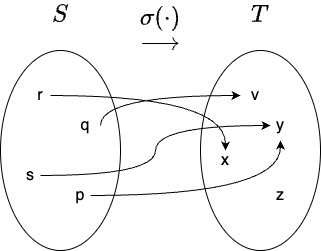
\includegraphics[width=0.45\textwidth]{Figures/Mappings_example.png}
    \caption{Mapping Example, arrows show how $\sigma$ operates on individual elements of $S$}
    \label{fig:simple_mapping_example}
\end{figure}

\begin{definition}[Image (of a set under a mapping)]
We may denote the \textit{image} of set $S$ under $\sigma$:
\begin{align}
    \text{The image of } S = \text{im} S= \{\sigma(s)|s\in S\}\nonumber
\end{align}
\end{definition} 
\begin{definition}[Pre-image (under a mapping)]
Element $s\in S$ is called a \textit{pre-image} of $t\in T$ if $\sigma(s)=t$
\end{definition}
%\noindent\textbf{Defn:} Element $s\in S$ is called a \textit{pre-image} of $t\in T$ if $\sigma(s)=t$\steezybreak\\
\begin{definition}[Inverse Image (of an element under a mapping)]
The \textit{inverse image} of $t$, denoted $\sigma^{-1}(t)$ is the set of all pre-images of $t$:
\begin{align}
    \sigma^{-1}(t)=\{s\in S | \sigma(s)=t \}\nonumber
\end{align}
\end{definition}
% \noindent\textbf{Defn:} The \textit{inverse image} of $t$, denoted $\sigma^{-1}(t)$ is the set of all pre-images of $t$:
% \begin{align}
%     \sigma^{-1}(t)=\{s\in S | \sigma(s)=t \}
% \end{align}
e.g. in Figure \ref{fig:simple_mapping_example} we have $\sigma^{-1}(x)=\{r\}$ and $\sigma^{-1}(y)=\{p,s\}$\\
Notice that a mapping is a special kind of relation, an equivalent definition for a mapping is as follows: A mapping from $S$ to $T$ is a subset $R\subset S \times T$ who has the property that $\forall s \in S, \exists \ \text{one and only one } t\in T \ni (s,t)\in R$, meaning that all members of the source set have a "representative" in the subset $R$, and that representative is paired with one and only one image $t\in T$. This view considers functions like lookup tables where the first entry of a given pair $(s,t)$ indicates the source element and the second entry represents the element he gets mapped to in $T$. The mapping in Figure \ref{fig:simple_mapping_example} could be written like so: $R=\{(r,x),(q,v),(s,y),(p,y)\} \subset S\times T$. When using this view, the subset of pairs, $R$, is referred to as the \textit{graph} of the mapping or function. 
\begin{notation}
When denoting mappings, Herstein prefers the notation $s\sigma$ rather than $\sigma(s)$ but the notations are related as follows: $\sigma(s) = s\sigma$, another example $\tau(a)=a\tau$, etc. 
\end{notation}

\noindent We will now present three important types of mappings.

\begin{definition}[Surjective, Injective, and Bijective Mappings]
\index{Surjective}
\index{Injective}
\index{Bijective}
\label{def:surj_inj_bij}
A mapping $\sigma: S\rightarrow T$ is \textit{surjective (a.k.a. onto)} if $\forall t\in T \ \exists \ s\in S \ni \sigma(s)=t$. (So $\sigma$ is surjective if every $t\in T$ has a pre-image)\steezybreak\\
A mapping $\sigma: S\rightarrow T$ is \textit{injective (a.k.a. one-to-one)} if $s_1\neq s_2 \implies \sigma(s_1)\neq \sigma(s_2)$. \\(So $\sigma$ is injective if distinct elements in $S$ \textit{stay} distinct when $\sigma$ is applied)\steezybreak\\
A mapping $\sigma: S\rightarrow T$ is \textit{bijective (a.k.a. a one-to-one correspondence)} if $\sigma$ is both injective \textit{and} surjective.\footnote{An injective mapping is often called an \textit{injection}\index{Injection}. A surjective mapping is often called a \textit{surjection}\index{Surjection}. A bijective mapping is often called a \textit{bijection}\index{Bijection}.}
\end{definition}
% \noindent\textbf{Defn:} A mapping $\sigma: S\rightarrow T$ is \textit{surjective (a.k.a. onto)} if $\forall t\in T \ \exists \ s\in S \ni \sigma(s)=t$. (So $\sigma$ is surjective if every $t\in T$ has a pre-image)\steezybreak\\
% A mapping $\sigma: S\rightarrow T$ is \textit{injective (a.k.a. one-to-one)} if $s_1\neq s_2 \implies \sigma(s_1)\neq \sigma(s_2)$. (So $\sigma$ is injective if distinct elements in $S$ \textit{stay} distinct when $\sigma$ is applied)\steezybreak\\
% A mapping $\sigma: S\rightarrow T$ is \textit{bijective (a.k.a. a one-to-one correspondence)} if $\sigma$ is both injective \textit{and} surjective.\steezybreak\\
\begin{definition}[Equality of Mappings (Equality of Functions)]
Mappings $\sigma : S \rightarrow T$ and $\tau: S \rightarrow T$ are equal if:
\begin{equation}
    \sigma(s)=\tau(s) \ \forall \ s\in S\nonumber
\end{equation}
\end{definition}
% \noindent\textbf{Defn:} Mappings $\sigma : S \rightarrow T$ and $\tau: S \rightarrow T$ are equal if:
% \begin{equation}
%     \sigma(s)=\tau(s) \ \forall \ s\in S\nonumber
% \end{equation}
\begin{definition}[Composition of mappings]
For mappings $\sigma: S\rightarrow T$, $\tau: T\rightarrow U$ the composition of $\sigma$ and $\tau$ is the mapping $\tau \circ \sigma: S\rightarrow U$ 
\begin{equation}
    (\tau \circ \sigma)(s) = \tau(\sigma(s)) \ \forall \ s \in S \nonumber
\end{equation}
\end{definition}
% \noindent\textbf{Defn:} For mappings $\sigma: S\rightarrow T$, $\tau: T\rightarrow U$ the composition of $\sigma$ and $\tau$ is the mapping $\tau \circ \sigma: S\rightarrow U$ 
% \begin{equation}
%     (\tau \circ \sigma)(s) = \tau(\sigma(s)) \ \forall \ s \in S \nonumber
% \end{equation}
\newpage
\begin{notation}
The symbol $\circ$ is commonly read ``after", so $\tau \circ \sigma$ would read ``tau after sigma" which makes sense when we think of wrapping functions around each other (tau gets applied after sigma gets applied), however Herstein prefers another convention that treats $\circ$ more like ``then".\steezybreak\\
Herstein writes the composition $(\tau \circ \sigma)(s)$ in this way: $ (s)(\sigma \circ \tau)$ so when reading Herstein notation we can think of $\circ$ as ``then" and it is essentially saying ``apply sigma to $s$, then apply tau). This can be confusing af but I will try to consistently use the ``after" notation because I like to think of $f(g(x))=(f\circ g) (x)$
\end{notation}

\subsection{Some Examples of Mappings}
\begin{example}
The Identity Map for set $S$,  $I_S: S\rightarrow S$ defined by $I_S(s)=s$, this mapping is also commonly written as just $I: S\rightarrow S$ (i.e. no subscript) when it is obvious which set's identity mapping we are referring to.
\end{example}
%\noindent\textbf{Example 1:} The Identity Map for set $S$,  $I_S: S\rightarrow S$ defined by $I_S(s)=s$, this mapping is also commonly written as just $I: S\rightarrow S$ (i.e. no subscript) when it is obvious which set's identity mapping we are referring to\steezybreak\\

\begin{example}
Below we give an example of composition of mappings where $S=T=U=\{1,2,3\}$ (see figure \ref{fig:composition_example} below)
%\textbf{Example 2:} Below we give an example of composition of mappings where $S=T=U=\{1,2,3\}$ (see figure \ref{fig:composition_example} below)
\begin{figure}[h!]
    \centering
    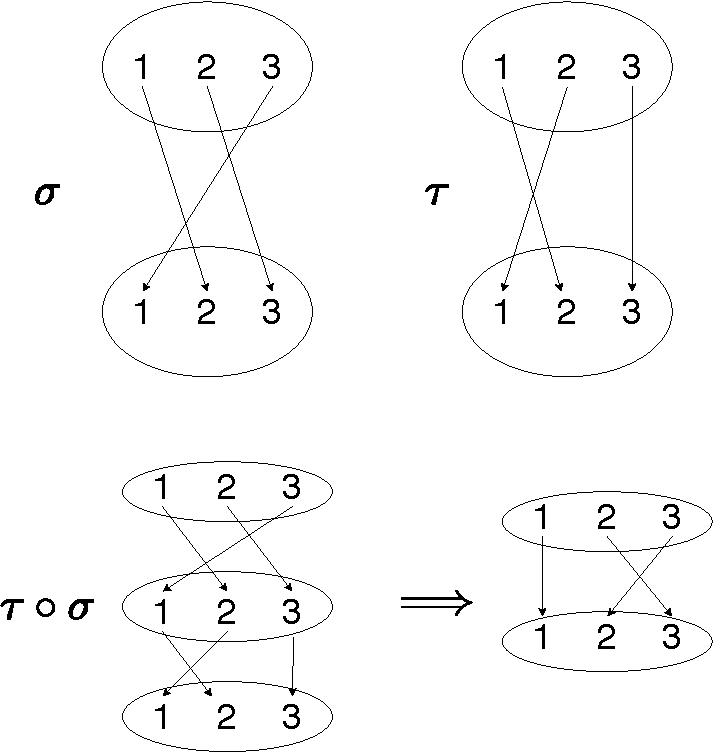
\includegraphics[width=0.75\textwidth]{Figures/composition_diagram-cropped.pdf}
    \caption{Composition Example (Ex 2) where $S=T=U=\{1,2,3\}$}
    \label{fig:composition_example}
\end{figure}
\end{example}
\noindent For example 3, we need one more definition.
\begin{definition}[Power set]
The \textit{power set} $S^{*}$ of a set $S$ is the collection of all subsets of $S$.
\end{definition}
%\noindent\textbf{Defn:} The power set $S^{*}$ of a set $S$ is the collection of all subsets of $S$.\steezybreak\\
\textbf{Example of a power set:} $S=\{1,2,3\}$ has power set $S^*=\{\{1\},\{2\},\{3\},\{2,3\},\{1,3\},\{1,2\},\emptyset,S\}$. If $S$ has $n$ elements, then $S^*$ has $2^n$ elements. \\
\noindent \textbf{\textit{Note(!):}} $S^{*}$'s elements are \textit{subsets} of $S$, not elements of $S$, e.g. $\{\{1\},\{2\}\}\neq \{1,2\}$ and $1\not \in \{\{1\},\{2\}\}$ but $1\in \{1,2\}$, the first set has elements that are \textit{subsets} (of numbers/integers) but the second set has elements that are \textit{numbers/integers}.
\begin{example}
The standard map from a set to its equivalence classes $\tilde{S}^*\subset S^*$.\\ 
Suppose $\sim$ is an equivalence relation on $S$, each equivalence class is a member of $S^*$. Define $\tau:S\rightarrow \tilde{S}^*$ by $\tau(s)=cl(s)$ (i.e. $\tau$ takes $s$ to the class in which it sits/belongs). This map is surjective but not injective.
\end{example}
% \noindent\textbf{Example 3:} The standard map from a set to its equivalence classes.\steezybreak\\
% Suppose $\sim$ is an equivalence relation on $S$, each equivalence class is a member of $S^*$. Define $\tau:S\rightarrow S^*$ by $\tau(s)=cl(s)$ (i.e. $\tau$ takes $s$ to the class in which it sits/belongs). This map is surjective but not injective.\steezybreak\\
% \textbf{Associative Law of Composition (Lemma 1.2.1)}\\
% If $\sigma:S\rightarrow T$ and $\tau: T \rightarrow U$ and $\mu: U \rightarrow V$, then:
% \begin{equation}
%     (\mu\circ\tau)\circ \sigma = \mu \circ (\tau \circ \sigma)\nonumber
% \end{equation}
% \textbf{Proof:} Pick arbitrary $s\in S$\\
% \begin{align}
%     [(\mu\circ \tau)\circ \sigma](s)&= (\mu\circ\tau)(\sigma(s))\nonumber \ \ \ \ \ \ \ (\text{since }(a\circ\sigma) (s) = a(\sigma(s)))\\
%     &= \mu[\tau(\sigma(s))]\nonumber \ \ \ \ \ \ \ \ \ \ (\text{since } \sigma(s)\in T \text{ and } (\mu \circ \tau)(t)= \mu(\tau(t)) \ \forall \ t \in T)\\
%     &= \mu[\tau\circ\sigma(s)]\nonumber \ \ \ \ \ \ \ \ \ \ (\text{since }  (\tau \circ \sigma)(s)= \tau(\sigma(s))  \in U ) \\
%     &= \mu\circ[\tau\circ\sigma(s)].\nonumber \  \ \ \ \ \ (\text{since }  (\mu\circ a)(u)= \mu(a(u))  )\ \ \ \ \ \ \ \blacksquare
% \end{align}
%\newpage
\begin{lemma}[Associative Law of Composition]
%\textbf{ (Lemma 1.2.1)}\\
If $\sigma:S\rightarrow T$ and $\tau: T \rightarrow U$ and $\mu: U \rightarrow V$, then:
\begin{equation}
    (\mu\circ\tau)\circ \sigma = \mu \circ (\tau \circ \sigma)\nonumber
\end{equation}
\textbf{Proof:} Pick arbitrary $s\in S$\\
\begin{align}
    [(\mu\circ \tau)\circ \sigma](s)&= (\mu\circ\tau)(\sigma(s))\nonumber \ \ \ \ \ \ \ (\text{since }(a\circ\sigma) (s) = a(\sigma(s)))\\
    &= \mu[\tau(\sigma(s))]\nonumber \ \ \ \ \ \ \ \ \ \ (\text{since } \sigma(s)\in T \text{ and } (\mu \circ \tau)(t)= \mu(\tau(t)) \ \forall \ t \in T)\\
    &= \mu[\tau\circ\sigma(s)]\nonumber \ \ \ \ \ \ \ \ \ \ (\text{since }  (\tau \circ \sigma)(s)= \tau(\sigma(s))  \in U ) \\
    &= \mu\circ[\tau\circ\sigma(s)].\nonumber \  \ \ \ \ \ (\text{since }  (\mu\circ a)(u)= \mu(a(u))  )\ \ \ \ \ \ \ \blacksquare
\end{align}
\end{lemma}
\begin{lemma}
If $\sigma: S\rightarrow T$, $\tau: T\rightarrow V$
\begin{enumerate}
    \item if both $\sigma$ and $\tau$ are surjective, then $\tau \circ \sigma$ is surjective.
    \item if both $\sigma$ and $\tau$ are injective, then $\tau \circ \sigma$ is injective.
\end{enumerate}
\textbf{Proof:} 1) We will begin by assuming $\sigma$ and $\tau$ are surjective and show this implies $\tau \circ \sigma$ is surjective. Assume $\sigma$ and $\tau$ surjective. Let $v\in V$, $\tau$ surjective means $\exists \ t\in T \ni \tau(t)=v $, similarly, $\sigma$ surjective $\implies$ $\exists \ s\in S \ni \sigma(s)=t$. Then
\begin{equation}
    (\tau \circ \sigma)(s)=\tau[\sigma(s)]=\tau[t]=v\nonumber
\end{equation}
so $s$ is a pre-image of $v$ meaning $\tau\circ \sigma$ is also surjective.

2) Take $s_1,s_2\in S \ni s_1\neq s_2$, then $\sigma$ injective $\implies$ $\sigma(s_1)\neq\sigma(s_2)$. $\tau$ injective $\implies \tau[\sigma(s_1)]\neq \tau[\sigma(s_2)] \implies (\tau \circ \sigma)$ keeps distinct elements distinct (so $\tau \circ \sigma$ is injective). $\blacksquare$
\end{lemma}
% \textbf{Lemma 1.2.2}\\
% If $\sigma: S\rightarrow T$, $\tau: T\rightarrow V$
% \begin{enumerate}
%     \item if both $\sigma$ and $\tau$ are surjective, then $\tau \circ \sigma$ is surjective.
%     \item if both $\sigma$ and $\tau$ are injective, then $\tau \circ \sigma$ is injective.
% \end{enumerate}
% \textbf{Proof:} 1) We will begin by assuming $\sigma$ and $\tau$ are surjective and show this implies $\tau \circ \sigma$ is surjective. Assume $\sigma$ and $\tau$ surjective. Let $v\in V$, $\tau$ surjective means $\exists \ t\in T \ni \tau(t)=v $, similarly, $\sigma$ surjective $\implies$ $\exists \ s\in S \ni \sigma(s)=t$. Then
% \begin{equation}
%     (\tau \circ \sigma)(s)=\tau[\sigma(s)]=\tau[t]=v\nonumber
% \end{equation}
% so $s$ is a pre-image of $v$ meaning $\tau\circ \sigma$ is also surjective.

% 2) Take $s_1,s_2\in S \ni s_1\neq s_2$, then $\sigma$ injective $\implies$ $\sigma(s_1)\neq\sigma(s_2)$. $\tau$ injective $\implies \tau[\sigma(s_1)]\neq \tau[\sigma(s_2)] \implies (\tau \circ \sigma)$ keeps distinct elements distinct (so $\tau \circ \sigma$ is injective). $\blacksquare$ \steezybreak\\
\begin{lemma}
$\sigma :S \rightarrow T$.
\begin{equation}
    \sigma \text{ is a bijection} \iff \exists \ \mu: T\rightarrow S \ni \mu\circ \sigma = I_S \text{ and } \sigma\circ \mu = I_T\nonumber
\end{equation}
(The method of proof for an equivalence $\Leftrightarrow$ is to show each side implies the other)\steezybreak\\
\textbf{Proof:} we will begin with showing the $\Leftarrow$ direction.\\
\textbf{$\Leftarrow$:} \\Assume that $\mu$ exists with the stated properties; show that this forces $\sigma$ to be a bijection. We will begin by showing $\sigma$ is injective through a contradiction \steezybreak\\
\textit{$\sigma$ Inj:} Suppose $\sigma$ is not injective $\implies \exists \ s_1,s_2\in S \ni s_1\neq s_2$ and $\sigma(s_1)=\sigma(s_2)$. But we know $\mu \circ \sigma = I_s$ which means $\mu\circ \sigma (s_1) = \mu\circ \sigma(s_2) = s_1=s_2$ $\Rightarrow\Leftarrow$ $s_1$ and $s_2$ were assumed non-equal!! So $\sigma$ must be injective.\steezybreak\\
Now, we will show that $\sigma$ is also surjective if such a $\mu$ exists.\steezybreak\\
\textit{$\sigma$ Surj:} Take arbitrary $t\in T$. $t= I_T(t)= (\sigma\circ\mu)(t)=\sigma(\mu(t))$ and $\mu(t)\in S$ so $\mu(t)$ serves as a preimage for $t$ under $\sigma$. Therefore $\sigma$ is surjective. \\ 

\noindent Now to show the other implication (i.e. show LHS of Lemma 1.2.3 $\implies$ RHS) \\
\textbf{$\Rightarrow$:} \\ We assume $\sigma$ is a bijection, now we have to:
\begin{enumerate}
    \item Define a rule called $\mu:T\rightarrow S$
    \item Show $\mu$ is a mapping (each element in $T$ should go to exactly one element in $S$)
    \item Verify the defined $\mu$ satisfies the stated composition properties
\end{enumerate}
\textbf{1)} Which element of $S$ should be $\mu(t)$? Well, $\sigma$ surjective $\implies t$ has a pre-image in $S$ or $\exists s\in S \ni \sigma(s)=t$. So let's define $ \mu: T\rightarrow S$ by $\mu(t)=s$ for which $\sigma(s)=t$ (i.e. $\mu(t)$ will always just take $t$ to its pre-image under $\sigma$)\steezybreak\\

\noindent\textbf{2)} Is $\mu$ well-defined (is $\mu$ actually a mapping/function)? Can $t$ have more than one pre-image (this would result in more than one value for $\mu(t)$ making $\mu$ not a function)?\steezybreak\\
NO! $t$ cannot have more than one pre-image because having $s_1\neq s_2$ and $\sigma(s_1)=\sigma(s_2)=t$ would violate injectivity of $\sigma$. So $\mu$ is well-defined.\steezybreak\\

\noindent\textbf{3)} Take $s\in S$, $(\mu\circ \sigma)(s)=\mu(\sigma(s))=\mu(t)=s=I_S(s)$. $\therefore (\mu\circ \sigma)= I_S$\steezybreak\\

Take $t\in T$, $(\sigma\circ \mu)(t)= \sigma(\mu(t))=\sigma(s)=t=I_T(t)$. $\therefore (\sigma\circ \mu) = I_T$. $\blacksquare$ \steezybreak\\

\noindent Notation: In light of its role, $\mu$ is renamed $\sigma^{-1}$ (``$\sigma$ inverse") and we can rewrite the lemma like this:

\begin{equation}
    \sigma:S\rightarrow T \text{ is a bijection } \iff \sigma \text{ has an inverse } \sigma^{-1}: T\rightarrow S \text{ with } (\sigma^{-1}\circ \sigma)= I_S \text{ and } (\sigma \circ \sigma^{-1})=I_T\nonumber
\end{equation}
\end{lemma}\steezybreak
\begin{tcolorbox}
\begin{center}
    $\star\star\star$ \textbf{Read up to this point to Complete Homework 1 (Located in \ref{sec:HW1})} $\star\star\star$
\end{center}
\end{tcolorbox}
\steezybreak
% \noindent\textbf{Lemma 1.2.3} $\sigma :S \rightarrow T$.
% \begin{equation}
%     \sigma \text{ is a bijection} \iff \exists \ \mu: T\rightarrow S \ni \mu\circ \sigma = I_S \text{ and } \sigma\circ \mu = I_T\nonumber
% \end{equation}
% (The method of proof for an equivalence $\Leftrightarrow$ is to show each side implies the other)\steezybreak\\
% \textbf{Proof:} we will begin with showing the $\Leftarrow$ direction.\\
% \textbf{$\Leftarrow$:} Assume that $\mu$ exists with the stated properties; show that this forces $\sigma$ to be a bijection. We will begin by showing $\sigma$ is injective through a contradiction \steezybreak\\
% \textit{$\sigma$ Inj:} Suppose $\sigma$ is not injective $\implies \exists s_1,s_2\in S \ni s_1\neq s_2$ and $\sigma(s_1)=\sigma(s_2)$. But we know $\mu \circ \sigma = I_s$ which means $\mu\circ \sigma (s_1) = \mu\circ \sigma(s_2) = s_1=s_2$ $\Rightarrow\Leftarrow$ $s_1$ and $s_2$ were assumed non-equal!! So $\sigma$ must be injective. Now we will show that $\sigma$ is also surjective if such a $\mu$ exists.\steezybreak\\
% \textit{$\sigma$ Surj:} Take arbitrary $t\in T$. $t= I_t(t)= (\sigma\circ\mu)(t)=\sigma(\mu(t))$ and $\mu(t)\in S$ so $\mu(t)$ serves as a preimage for $t$ under $\sigma$. Therefore $\sigma$ is surjective. \steezybreak\\

% \noindent Now to show the other implication (LHS of Lemma 1.2.3 $\implies$ RHS) \steezybreak\\
% \textbf{$\Rightarrow$:}Now we assume $\sigma$ is a bijection, now we have to:
% \begin{enumerate}
%     \item Define a rule called $\mu:T\rightarrow S$
%     \item Show $\mu$ is a mapping (each element in $T$ should go to exactly one element in $S$)
%     \item Verify the defined $\mu$ satisfies the stated composition properties
% \end{enumerate}
% \textbf{1)} Which element of $S$ should be $\mu(t)$? Well, $\sigma$ surjective $\implies t$ has a preimage in $S$ or $\exists s\in S \ni \sigma(s)=t$. So let's define $ \mu: T\rightarrow S$ by $\mu(t)=s$ for which $\sigma(s)=t$ (i.e. $\mu(t)$ will always just take $t$ to its preimage under $\sigma$)\steezybreak\\

% \noindent\textbf{2)} Is $\mu$ well defined? (Is it actually a mapping/function?). Can $t$ have more than one pre-image (this would result in more than one value for $\mu(t)$ making $\mu$ not a function)?\steezybreak\\
% NO! Because having $s_1\neq s_2$ and $\sigma(s_1)=\sigma(s_2)$ would violate injectivity of $\sigma$. So $\mu$ is well-defined.\steezybreak\\

% \noindent\textbf{3)} Take $s\in S$, $(\mu\circ \sigma)(s)=\mu(\sigma(s))=\mu(t)=s=I_s(s)$. $\therefore (\mu\circ \sigma)= I_S$\steezybreak\\

% Take $t\in T$, $(\sigma\circ \mu)(t)= \sigma(\mu(t))=\sigma(s)=t=I_T(t)$. $\therefore (\sigma\circ \mu) = I_T$. $\blacksquare$ \steezybreak\\

% \noindent Notation: In light of its role, $\mu$ is renamed $\sigma^{-1}$ (``$\sigma$ inverse") and we can rewrite the lemma like this:

% \begin{equation}
%     \sigma:S\rightarrow T \text{ is a bijection } \iff \sigma \text{ has an inverse } \sigma^{-1}: T\rightarrow S \text{ with } (\sigma^{-1}\circ \sigma)= I_S \text{ and } (\sigma \circ \sigma^{-1})=I_T\nonumber
% \end{equation}

\section{\texorpdfstring{The Integers (in examples, $a,b,c...\in \mathbb{Z}$)}{The Integers (in examples, a,b,c... elements of Z (the integers)}}
\label{sec:TheIntegers}
\textbf{Euclidean Algorithm (Axiom):} Given $a$ and $b\neq 0$, $\exists \ q,r \in \mathbb{Z}\ni a= bq+r$ where $0\leq r<|b|$  \\  
We call $b$ the divisor, $q$ the quotient, and $r$ the remainder.\steezybreak\\
\textbf{Examples:}
\begin{example}
\setstackgap{S}{1.5pt}
\stackMath\def\stackalignment{r}
Let $a=143$ and $b=20$\steezybreak\\
\(
\stackunder{%
  20 \stackon[1pt]{\showdiv{143}}{7}%
}{%
  \Shortstack[l]{{\ph{3}\underline{140}} \ph{300}3}%
}
\) $\implies \ \ a=bq+r=143=(20)(7) + 3$ \\
\end{example}

\begin{example}
How about $a=-143$ and $b=20$?

\(
\stackunder{%
  20 \stackon[1pt]{\showdiv{-143}}{-7}%
}{%
  \Shortstack[l]{{\ph{300}\underline{-140}} \ph{3000}-3}%
}
\)   \ \ \ \     !!! not a valid division since $-3$ doesn't fall between 0 and 19... let's try again \smiley \\

\(
\stackunder{%
  20 \stackon[1pt]{\showdiv{-143}}{-8}%
}{%
  \Shortstack[l]{{\ph{000}\underline{-160}} \ph{50000}17}%
}
\)$\implies \ \ a=bq+r=-143=(20)(-8) + 17$ \\
\end{example}

\begin{example}

\noindent How about $a=143$ and $b=-20$?\steezybreak\\
\(
\stackunder{%
  -20 \stackon[1pt]{\showdiv{143}}{-7}%
}{%
  \Shortstack[l]{{\ph{3000}\underline{140}} \ph{300000}3}%
}
\) $\implies \ \ a=bq+r=143=(-20)(-7) + 3$
\steezybreak\\ \\
\begin{definition}[Divides (relation)]
$b\in \Z \ni b\neq 0$. $b$ \textit{divides} $a$ (denoted $b|a$) if $\exists \ m\in \mathbb{Z}\ni a=mb$
\steezybreak\\
\noindent (Note, under Eucl., if $a=b\cdot q + r, \ \ 0\leq r<|b|, \ b\neq 0$, then $b|a \iff r=0$)
\end{definition}
\end{example}

%\noindent\textbf{Defn:} $b\in \Z \ni b\neq 0$. $b$ divides $a$ (denoted $b|a$) if $\exists \ m\in \mathbb{Z}\ni a=mb$ \steezybreak\\
\noindent Here are some useful observations we can make from this new definition.\steezybreak\\
\noindent\textbf{Observation 1:} $b|1\implies b=\pm 1$\\
\textit{Proof:} $b|1$ means $\exists m\in \mathbb{Z}\ni 1=mb$. There are only 2 possible combinations of integers that satisfy $mb=1$, either $m=b=1$ (i.e. $(1)(1)=1$) or $m=b=-1$ (i.e. $(-1)(-1)=1$) $\implies b=\pm 1$ \steezybreak\\
\noindent\textbf{Observation 2:} $a|b$ and $b|a$ $\implies$ $b=\pm a$ \steezybreak\\
\textit{Proof:} $a|b \implies \exists m \in \mathbb{Z} \ni b= ma$. $b|a \implies \exists n \in \mathbb{Z} \ni a= nb$. So $b=ma=mnb$. The first and last expressions ($b=mnb$) imply that $mn=1$, using our previous observation, this forces $m=\pm 1$ $\implies$ $b=\pm a$\steezybreak\\
\noindent\textbf{Observation 3:} $b|0$ is true for any non-zero $b\in \mathbb{Z}$ because $0=0\cdot b$ is an integer multiple of $b$ ($0\in \mathbb{Z}$ is the integer multiple)\steezybreak\\
\noindent\textbf{Observation 4:}  $b|a$ and $b|c$ $\implies$ $b|(\text{any linear combination of }a,c)$ \steezybreak\\
\textit{Proof:} 
\begin{align}
    b|a &\implies \ \ \exists \ m \in \Z \ni a=mb \nonumber \\
    b|c &\implies \ \ \exists \ n \in \Z \ni c=nb \nonumber
\end{align}
Take $r,s\in \Z$, then $ra+sc$ is an arbitrary linear combination of $a,c$.
\begin{align}
    ra+sc=r(mb)+s(nb)=(rm+sn)b\nonumber
\end{align}
lastly we note $(rm+sn)\in \Z$, $\therefore b|(ra+sc)$.
\noindent Ver nice. Ok, lets put these observations in one place for quick reference
\begin{proposition}[Four Observations about Integer Division] 
For integers $b\neq 0$
\begin{enumerate}
    \item $b|1\implies b=\pm 1$
    \item $a|b$ and $b|a$ $\implies b=\pm a$
    \item $b|0 \ \forall \ b \in \Z \ni b\neq 0$
    \item $b|a$ and $b|c$ $\implies$ $b|(ra+sc) \ \forall \ r,s \in \Z$
\end{enumerate}
\end{proposition}
% \noindent\textbf{Four Observations about Division}
% \begin{enumerate}
%     \item $b|1\implies b=\pm 1$
%     \item $a|b$ and $b|a$ $\implies b=\pm a$
%     \item $b|0 \ \forall \ b \in \Z \ni b\neq 0$
%     \item $b|a$ and $b|c$ $\implies$ $b|(ra+sc) \ \forall \ r,s \in \Z$
% \end{enumerate}

\subsection{Dividing Integers and Greatest Common Divisors}
What is the greatest common divisor of $24$ and $36$? Let's list the divisors they have in common:
\begin{equation}
    \pm 1, \pm 2, \pm 3, \pm 4, \pm 6, \pm 12 \nonumber
\end{equation}
Well that seems to be all of them, so the greatest common divisor is the biggest: $12$\steezybreak\\
\begin{definition}[Greatest Common Divisor]
The positive integer $c$ is the \textit{greatest common divisor} of $a$ and $b$ denoted $GCD(a,b)$ provided:
\begin{enumerate}[label=\roman*)]
    \item $c|a$ and $c|b$      \ \ \ \ \ \ \ \ \ \ \ \ \ \ \ \ \ \ \ \ \ \ \ (common)
    \item if $d|a$ and $d|b$, then $d|c$ \ \ \ \ \ \  (biggest)
\end{enumerate}
\end{definition}
% \noindent\textbf{Defn:} The positive integer $c$ is the greatest common divisor of $a$ and $b$ denoted $GCD(a,b)$ provided:
% \begin{enumerate}[i)]
%     \item $c|a$ and $c|b$      (common)
%     \item if $d|a$ and $d|b$, then $d|c$  (biggest)
% \end{enumerate}
\textit{Note:} For the readers who are reviewing with this text and already know some category theory, does the definition of GCD look familiar? Can you think of a category $\mathcal{C}$ where GCD is a categorical product? Using similar reasoning, what must the co-product be in this category? Does this category have a terminal or initial object(s)? If so, what? (hint: $\text{obj}(\mathcal{C})=\Z^+$)
\begin{proposition}[Uniqueness of $GCD(a,b)$]
Suppose $c_1$ and $c_2$ both satisfy the definition of $GCD(a,b) \implies c_1|c_2$ and $c_2|c_1$, so by observation \#2, $c_1=\pm c_2 \implies c_1=c_2$ (because, $c_1,c_2$ assumed positive). So the $GCD(a,b)$ is unique.
\end{proposition}
\begin{example}
$GCD(0,0)$ Does not exist (DNE)
\end{example}
\begin{example}
$GCD(0,7)=7$ because $0$ and $7$ have common factors $\pm 1,\pm 7$; \\
In fact: $GCD(0, b)=|b| \ \ \forall \ b\in \Z\ni b\neq 0$.
\end{example}


\begin{lemma}[Existence of $GCD(a,b)$] 
if $a,b\in \Z$ are not both $0$, then $GCD(a,b)$ exists; in fact, $\exists \ m_0,n_0\in \Z \ni $
\begin{equation}
    GCD(a,b)=m_0 a+n_0 b\nonumber
\end{equation}

\noindent\textbf{Proof:} Let $M= \{ma+nb \ | \ \forall \ m,n,\in \Z \}$
\begin{align}
a&=(1)\cdot a + (0)\cdot b \in M \nonumber \\
b&=(0)\cdot a + (1)\cdot b \in M\nonumber \\
-a&=(-1)\cdot a + (0)\cdot b \in M\nonumber \\
-b&=(0)\cdot a + (-1)\cdot b \in M\nonumber 
\end{align}
At least one of $a,-a,b,-b$ is positive so we may say that $M$ contains positive integers. Let $c$ denote the smallest positive integer in $M$. Then:\\
\begin{equation}
    c=m_0 a +n_0 b \ \ \text{ for some } m_0,n_0\in \Z \nonumber
\end{equation}
\textit{Claim:} $c=GCD(a,b)$. ( to prove this claim we must show $c|a$, $c|b$, and if $d|a$ and $d|b$ then $d|c$.)\\
\textit{Proof:} To begin we note that the Euclidean algorithm can be used to divide any element $\in M$ by $c$. Take arbitrary $m,n \in \Z$, then $ma+nb$ is an arbitrary element of $M$. Eucl. Algorithm $\implies$ $\exists q,r \in \Z\ni (ma+nb)=q\cdot c + r$ where $0\leq r < c$. Now we solve for $r$:
\begin{align}
    r&= (ma+nb)-q\cdot c \nonumber\\
    &= (ma+nb)-q(m_0a +n_0 b) \nonumber\\
    &= (m-qm_0)a+(n- q n_0)b \nonumber\\
    &\therefore r\in M \nonumber
\end{align}
Since $c$ is the \textit{smallest positive integer} in $M$, and $0\leq r < c$ and $r\in M$, this implies that $r=0$.\steezybreak\\
So $c|(ma+nb)$. If $c$ divides everything in $M$, then $c|a$ and $c|b$. Also if $d|a$ and $d|b$ then observation \#4 $\implies$ $d|(\text{the linear combination } m_0a+n_0b)$\steezybreak\\
$\therefore GCD(a,b)=c=m_0a+n_0b \ \ \ \ \blacksquare$\steezybreak\\
\end{lemma}
% \textbf{Lemma 1.3.1 (Existence of $GCD(a.b)$):} if $a,b\in \Z$ are not both $0$, then $GCD(a,b)$ exists; in fact, $\exists \ m_0,n_0\in \Z \ni $\\
% \begin{equation}
%     GCD(a,b)=m_0 a+n_0 b\nonumber
% \end{equation}

% \noindent\textbf{Proof:} Let $M= \{ma+nb|\forall m,n,\in \Z \}$\steezybreak\\
% $a=(1)\cdot a + (0)\cdot b \in M$\\
% $b=(0)\cdot a + (1)\cdot b \in M$\\
% $-a=(-1)\cdot a + (0)\cdot b \in M$\\
% $-b=(0)\cdot a + (-1)\cdot b \in M$\\

% At least one of $a,-a,b,-b$ is positive so we may say that $M$ contains positive integers. Let $c$ denote the smallest positive integer in $M$. Then:\\
% \begin{equation}
%     c=m_0 a +n_0 b \ \ \text{ for some } m_0,n_0\in \Z \nonumber
% \end{equation}
% \textit{Claim:} $c=GCD(a,b)$. ( to prove this claim we must show $c|a$, $c|b$, and if $d|a$ and $d|b$ then $d|c$.)\\
% \textit{Proof:} To begin we note that the Euclidean algorithm can be used to divide any element $\in M$ by $c$. Take arbitrary $m,n \in \Z$, then $ma+nb$ is an arbitrary element of $M$. Eucl. Algorithm $\implies$ $\exists q,r \in \Z\ni (ma+nb)=q\cdot c + r$ where $0\leq r < c$. Now we solve for $r$:
% \begin{align}
%     r&= (ma+nb)-q\cdot c \nonumber\\
%     &= (ma+nb)-q(m_0a +n_0 b) \nonumber\\
%     &= (m-qm_0)a+(n- +q n_0)b \nonumber\\
%     &\therefore r\in M
% \end{align}
% Since $c$ is the \textit{smallest positive integer} in $M$, and $0\leq r < c$ and $r\in M$, this implies that $r=0$.\steezybreak\\
% So $c|(ma+nb)$. If $c$ divides everything in $M$, then $c|a$ and $c|b$. Also if $d|a$ and $d|b$ then observation \#4 $\implies$ $d|(\text{the linear combination } m_0a+n_0b)$\steezybreak\\
% $\therefore GCD(a,b)=c=m_0a+n_0b \ \ \ \ \blacksquare$\steezybreak\\
\begin{example}
Find $GCD(1812,1200)$, to do this, we can use the euclidean algorithm to find GCD by first dividing $a$ by $b$ and then continually dividing the divisor by the remainder (Note: here we will represent $a$ as $a=qb+r$, i.e. writing the quotient first, this is allowed because integers are commutative under multiplication, this view is convenient for the next few examples):
\begin{align}
    1812 &=1\cdot1200+612\nonumber\\
    1200 &=1\cdot612+588 \nonumber\\
    612 &=1\cdot588+24 \nonumber\\
    588 &=24\cdot24+12 \nonumber\\
    24 &=2\cdot12+0 \nonumber
\end{align}
The GCD will be the second to last remainder (last remainder is always 0, i.e. you are done when the remainder =0) so in this case the GCD is $12$. This method is nice because reading these divisions from bottom to top ($\big\uparrow$) shows $12$ is a common divisor of $a$ and $b$ and reading from top to bottom ($\big\downarrow$) shows it is the greatest (since we stop the first time a zero remainder [i.e. a common divisor] appears).
\end{example}
% \textbf{Example 1} Find $GCD(1812,1200)$, to do this, we can use the euclidean algorithm to find GCD by first dividing $a$ by $b$ and then continually dividing the divisor by the remainder:
% \begin{align}
%     1812 &=1\cdot1200+612\nonumber\\
%     1200 &=1\cdot612+588 \nonumber\\
%     612 &=1\cdot588+24 \nonumber\\
%     588 &=24\cdot24+12 \nonumber\\
%     24 &=2\cdot12+0 \nonumber\\
% \end{align}
% The GCD will be the second to last remainder (last remainder is always 0, i.e. you are done when the remainder =0) so in this case the GCD is $12$. This method is nice because reading these divisions from bottom to top ($\big\uparrow$) shows $12$ is a common divisor of $a$ and $b$ and reading from top to bottom ($\big\downarrow$) shows it is the greatest (since we stop the first time a zero remainder [i.e. a common divisor] appears).\steezybreak\\
\begin{example}
Find $m,n\in \Z \ni GCD(71,31)=m\cdot 71+n\cdot 31$.\steezybreak\\
\begin{align}
    71&= 2\cdot 31+9 \ \implies 9=71-2\cdot 31 \nonumber\\
    31&= 3\cdot 9+4 \ \implies 4=31-3\cdot 9\nonumber\\
    9&= 2\cdot 4+1 \ \implies 1=9-2\cdot 4\nonumber\\
    4&= 4\cdot 1+0 \nonumber
\end{align}
So the $GCD(71,31)=1$ and using the implications we gathered along the way we can back-substitute for an expression in terms of $71$ and $31$
\begin{align}
    1&=9-2[31-3\cdot 9]\nonumber \\
    &=7\cdot 9- 2\cdot 31\nonumber \\
    &=7\cdot [71-2\cdot 31]- 2\cdot 31\nonumber \\
    &=7\cdot 71+ (-16)\cdot 31\nonumber 
\end{align}
\end{example}
% \noindent \textbf{Example 2} Find $m,n\in \Z \ni GCD(71,31)=m\cdot 71+n\cdot 31$.\steezybreak\\
% \begin{align}
%     71&= 2\cdot 31+9 \ \implies 9=71-2\cdot 31 \nonumber\\
%     31&= 3\cdot 9+4 \ \implies 4=31-3\cdot 9\nonumber\\
%     9&= 2\cdot 4+1 \ \implies 1=9-2\cdot 4\nonumber\\
%     4&= 4\cdot 1+0 \nonumber\\
% \end{align}
% So the $GCD(71,31)=1$ and using the implications we gathered along the way we can back-substitute for an expression in terms of $71$ and $31$
% \begin{align}
%     1&=9-2[31-3\cdot 9]\nonumber \\
%     &=7\cdot 9- 2\cdot 31\nonumber \\
%     &=7\cdot [71-2\cdot 31]- 2\cdot 31\nonumber \\
%     &=7\cdot 71+ (-16)\cdot 31\nonumber \\
% \end{align}
\newpage
\subsection{Alternate Method with $2\times 2$ Matrices}
Rather than performing repeated back-substitutions, there is a clean way we can implement this same procedure using $2\times 2$ matrices. Using our example from before,\\
\begin{align}
    71&= 2\cdot 31+9 \ \ \ \ \text{Let's denote }2=q_1\nonumber\\
    31&= 3\cdot 9+4 \ \ \ \ \ \ \text{Let's denote }3=q_2\nonumber\\
    9&= 2\cdot 4+1 \ \ \ \ \ \ \text{Let's denote }2=q_3 \ \text{ (don't use 0 remainder quotient)}\nonumber\\ \hline
    4&= 4\cdot 1+0 \nonumber
\end{align}
In this approach, instead of repeatedly back-substituting ourselves, we take a consecutive product of matrices whose values are determined by the quotients we discover by running the eucl. alg. The matrices will have the form:
\begin{equation}
   M=
  \left( {\begin{array}{cc}
   0 & 1 \\
   1 & -q \\
  \end{array} } \right)
\nonumber
\end{equation}
\textbf{Ex:}
\begin{align}
  \left( {\begin{array}{cc}
   0 & 1 \\
   1 & -q_3 \\
  \end{array} } \right)\left( {\begin{array}{cc}
   0 & 1 \\
   1 & -q_2 \\
  \end{array} } \right)\left( {\begin{array}{cc}
   0 & 1 \\
   1 & -q_1 \\
  \end{array} } \right) 
  =\left( {\begin{array}{cc}
   0 & 1 \\
   1 & -2 \\
  \end{array} } \right)\left( {\begin{array}{cc}
   0 & 1 \\
   1 & -3 \\
  \end{array} } \right)\left( {\begin{array}{cc}
   0 & 1 \\
   1 & -2 \\
  \end{array} } \right)=\left( {\begin{array}{cc}
   -3 & 7 \\
   7 & -16 \\
  \end{array} } \right) \nonumber\\
  \therefore 1= (7)*71+(-16)*31
\nonumber
\end{align}
Why does this work? Consider again the equation:
\begin{align}
    a=qb+r \nonumber
\end{align}

when finding the GCD, we begin by dividing $a$ by $b$ and recording the quotient and remainder that solved the above equation, we then replace our divisor with the last remainder and $a$ with the last divisor and continue in this way until we find a remainder that is equal to $0$., i.e. we enforce:
\begin{align}
    a_0=a, d_0=b \ \ \ (a\text{ and divisor }b)\nonumber\\
    d_{n+1}= r_n  \ \ \ (\text{ next divisor last remainder })\nonumber \\
    a_{n+1}= d_n \ \ \ (\text{ next dividend is last divisor })\nonumber 
\end{align}
One step of these divisions could be represented in matrix notation by using the following,
\begin{equation}
  \left( {\begin{array}{cc}
   0 & 1 \\
   1 & -q \\
  \end{array} } \right)\left( {\begin{array}{c}
   a\\
   b
  \end{array} } \right)=\left( {\begin{array}{c}
   b\\
   r
  \end{array} } \right)
\nonumber
\end{equation}
We can see that if we record the quotients as we go through the process, we can immediately find the linear combination that gives us the $GCD(a,b)$ in terms of $a$ and $b$ because it will simply be the coefficients in the last row of the product of these quotient matrices (i.e. $M$-like matrices).

\subsection{Primes and Prime Factorization of Integers}
\begin{definition}[Prime Numbers and Co-prime (Relatively prime) Pairs of Numbers]
\begin{enumerate}
    \item $a$ and $b$ are \textit{relatively prime} if $GCD(a,b)=1$.
    \item $p>1$ is \textit{prime} if its \textit{only} divisors are $\pm 1$ and $\pm p$.
\end{enumerate}
\end{definition}
% \textbf{Defn (s):}
% \begin{enumerate}
%     \item $a$ and $b$ are relatively prime if $GCD(a,b)=1$.
%     \item $p>1$ is prime if its \textit{only} divisors are $\pm 1$ and $\pm p$.
% \end{enumerate}
\begin{proposition}[a.k.a. Proposition $\star$] 
$p$ is prime $\iff$ $\forall \ n \in \Z $, either $p|n$ or $p$ and $n$ are relatively prime.\\
\textit{Proof:} \\
\textbf{$\Rightarrow :$}\\
Assume $p$ is prime; take arbitrary $n\in\Z$, $GCD(p,n)|p\ \ \implies \ GCD(p,n)$ is $1$ or $p$. If $GCD(p,n)=1$ then we are done since $p,n$ are relatively prime, if $GCD(p,n)=p$ then because $GCD(p,n)|n$ we have $p|n$.\steezybreak\\
\textbf{$\Leftarrow :$}\\
Assume $\forall n \in \Z$, either $p|n$ or $GCD(p,n)=1$. We must show that the only divisors of $p$ are $\pm 1, \pm p$. Let $d$ be a divisor of $p$ (so $d|p$). If we consider our hypothesis again, now thinking of $d$ as one of the $n\in\Z$ we have that either $p|d$ or $GCD(p,d)=1$. If $p|d$ then observation \#2 $\implies$ $d=\pm p$. If $GCD(p,d)=1$ then since $d$ is a common divisor of both $p$ (by assumption on $d$) and $d$ (obvious) and because the $GCD(p,d)$ is the greatest such divisor we have that $d|GCD(p,d)=d|1$ so by observation \# 1 we can conclude $d=\pm 1$. $\therefore \ p$ is prime. $\blacksquare$
\end{proposition}
% \textbf{Proposition $\star$:} $p$ is prime $\iff$ $\forall \ n \in \Z $, either $p|n$ or $p$ and $n$ are relatively prime.\\
% \textit{Proof:} \\
% \textbf{$\Rightarrow :$}\\
% Assume $p$ is prime; take arbitrary $n\in\Z$, $GCD(p,n)|p\ \ \implies \ GCD(p,n)$ is $1$ or $p$. If $GCD(p,n)=1$ then we are done since $p,n$ are relatively prime, if $GCD(p,n)=p$ then because $GCD(p,n)|n$ we have $p|n$.\steezybreak\\
% \textbf{$\Leftarrow :$}\\
% Assume $\forall n \in \Z$, either $p|n$ or $GCD(p,n)=1$. We must show that the only divisors of $p$ are $\pm 1, \pm p$. Let $d$ be a divisor of $p$ (so $d|p$). If we consider our hypothesis again, now thinking of $d$ as one of the $n\in\Z$ we have that either $p|d$ or $GCD(p,d)=1$. If $p|d$ then observation \#2 $\implies$ $d=\pm p$. If $GCD(p,d)=1$ then since $d$ is a common divisor of both $p$ (by assumption on $d$) and $d$ (obvious) and because the $GCD(p,d)$ is the greatest such divisor we have that $d|GCD(p,d)=d|1$ so by observation \# 1 we can conclude $d=\pm 1$. $\therefore \ p$ is prime. $\blacksquare$\steezybreak\\
\begin{lemma}
If $a$ is relatively prime to $b$ and $a|(b\cdot c)$, then $a|c$. \\
\textit{Proof:} $a,b$ rel. prime $\implies$ $GCD(a,b)=1$, by Lemma 1.3.1 $\exists m,n \in \Z \ni 1= GCD(a,b)=ma+nb$. Now if we multiply both sides of this expression by $c$ we have:
\begin{align}
    c=mac+nbc\nonumber
\end{align}
Now, certainly $a|a$, and from our hypothesis we have that $a|(bc)$ so by observation \# 4 about divisions, $a|(m\underline{a}c+ n\underline{bc})$, i.e. $a|c \ \ \blacksquare$ \steezybreak\\
\end{lemma}
% \noindent \textbf{Lemma 1.3.2:} If $a$ is relatively prime to $b$ and $a|(b\cdot c)$, then $a|c$. \\
% \textit{Proof:} $a,b$ rel. prime $\implies$ $GCD(a,b)=1$, by Lemma 1.3.1 $\exists m,n \in \Z \ni 1= GCD(a,b)=ma+nb$. Now if we multiply both sides of this expression by $c$ we have:
% \begin{align}
%     c=mac+nbc\nonumber
% \end{align}
% Now, certainly $a|a$, and from our hypothesis we have that $a|(bc)$ so by observation \# 4 about divisions, $a|(m\underline{a}c+ n\underline{bc})$, i.e. $a|c \ \ \blacksquare$ \steezybreak\\
\setcounter{dummy_lemma}{1}
\begin{corollary}
If $p$ is prime and $p|n_1n_2...n_K,\ \ n_i\in \Z$, then $p|n_i$ for at least one $i \in \{1,2,3,...,K\}$.\\
\textit{Proof:} By Prop. $\star$, either $p|n_1$ or $GCD(p,n_1)=1$. If $GCD(p,n_1)=1$ then Lemma 1.3.2 $\implies$ $p|n_2n_3...n_K$. Continue applying $\star$, if $GCD(p,n_i)=1$ for all $i$'s up to $K-1$ (i.e. $\forall \ 1\leq i\leq K-1$), then by Lemma 1.3.2 $p|n_K\ \ \ \ \blacksquare$
\end{corollary}
% \noindent\textbf{Corollary:} If $p$ is prime and $p|n_1n_2...n_K,\ \ n_i\in \Z$, then $p|n_i$ for at least one $i \in \{1,2,3,...,K\}$.\\
% \textit{Proof:} By prop $\star$, either $p|n_1$ or $GCD(p,n_1)=1$. If $GCD(p,n_1)=1$ then Lemma 1.3.2 $\implies$ $p|n_2n_3...n_K$. Continue applying $\star$, if $GCD(p,n_i)=1$ for all $i$'s up to $K-1$ (i.e. $\forall \ 1\leq i\leq K-1$), then by Lemma 1.3.2 $p|n_K\ \ \ \ \blacksquare$ \steezybreak\\
\setcounter{dummy}{0}
\begin{theorem}[Unique Factorization] 
Any integer $a>1$ can be factorized uniquely:
\begin{align}
    a=p_1^{\alpha_1}p_2^{\alpha_2}p_3^{\alpha_3}...p_t^{\alpha_t}\nonumber
\end{align}
Where $p_1>p_2>p_3>...>p_t$ are primes for each $\alpha_i>0$.\steezybreak\\
\noindent\textit{Proof:} We will hold off on the proof of this for now and we will prove it later in greater generality.\steezybreak\\
\end{theorem}

\textbf{Example:} $2520=60\cdot 42 = 7^1\cdot 5^1\cdot 3^2 \cdot 2^3$. 
\subsection{Congruence Mod N}
\begin{definition}[Congruence mod N]
$n\in \Z$; $a$ is \textit{congruent} to $b$ modulo $n$ iff $n|a-b$.\\
\textit{Notation:} 
\begin{align}
    a\equiv b \mod n &\iff n|(a-b) \nonumber \\
    &\iff \exists \ m\in \Z \ni a-b=mn \ \ \ (\text{i.e. } a=b+mn) \nonumber \\
    &\iff a \text{ is } b \text{ plus an integer multiple of } n \nonumber
\end{align}
\end{definition}
% \textbf{Defn:} $n\in \Z$; $a$ is congruent to $b$ modulo $n$ iff $n|a-b$.\\
% \textit{Notation:} 
% \begin{align}
%     a\equiv b \mod n &\iff n|(a-b) \nonumber \\
%     &\iff \exists \ m\in \Z \ni a-b=mn \ \ \ (\text{i.e. } a=b+mn) \nonumber \\
%     &\iff a \text{ is } b \text{ plus an integer multiple of } n \nonumber
% \end{align}
\begin{example}
Which integers $a$ are congruent to $26$ mod $12$? Well the last line in the definition above says we just need to take all the integer multiples of 12 (i.e. $12\Z$) and add $26$ to each:
\begin{align}
    12\Z= \{...,-36,-24,-12,0,12,24,36,...\}\nonumber\\
    12\Z+26= \{...,-10,2,14,26,38,50,62,...\}\nonumber
\end{align}
\textit{Notation:} To express that $-10$ is in the list we write:
\begin{equation}
    -10\equiv 26 \mod 12 \nonumber
\end{equation}
\end{example}
% \textbf{Example: } $26 \mod 12$, what integers are congruent to $26$ mod $12$? Take multiples of 12 (i.e. $12\Z$) and add $26$ to each:
% \begin{align}
%     12\Z= \{...,-36,-24,-12,0,12,24,36,...\}\nonumber\\
%     12\Z+26= \{...,-10,2,14,26,38,50,62,...\}\nonumber
% \end{align}
% \textit{Notation:} To express that $-10$ is in the list we write:
% \begin{equation}
%     -10\equiv 26 \mod 12 \nonumber
% \end{equation}
\begin{lemma}[Part 1] 
Congruence mod $n$ is an equivalence relation on the integers.\steezybreak\\
\textit{Proof:} Let $a,b,c\in \Z$
\begin{enumerate}
    \item \textit{Reflexivity:} $a\equiv a\mod n \iff n|(a-a) \iff n|0$. By observation \# 3, $n|0$\\
    $\therefore a\equiv a\mod n$\\
    $\therefore \ \ \ \equiv \mod n$ is reflexive\\
    \item \textit{Symmetry:} \\
    $a\equiv b\mod n \iff n|(a-b) \iff \exists \ k \in \Z \ni a-b=k\cdot n \iff b-a=(-k)\cdot n \ \ \ (\text{note } -k\in \Z) \implies n|(b-a)$\\
    $\therefore \ b\equiv a \mod n$
    \item \textit{Transitivity:} Assume $a\equiv b \mod n$ and $b\equiv c\mod n$. This implies two things:
    \begin{align}
        a\equiv b\mod n \iff n|(a-b) \nonumber\\
        b\equiv c\mod n \iff n|(b-c) \nonumber
    \end{align}
    Using these together with observation \# 4 we see $\implies$ $n|(a-b)+(b-c)=a-c$\\
    $\therefore a\equiv c \mod n.\ \ \ \ \ \ \blacksquare$
\end{enumerate}
\end{lemma}
% \textbf{Lemma 1.3.3 (Pt. 1):} Congruence mod $n$ is an equivalence relation on the integers.\steezybreak\\
% \textit{Proof:} Let $a,b,c\in \Z$
% \begin{enumerate}
%     \item \textit{Reflexivity:} $a\equiv a\mod n \iff n|(a-a) \iff n|0$. By observation \# 3, $n|0$\\
%     $\therefore a\equiv a\mod n$\\
%     $\therefore \ \ \ \equiv \mod n$ is reflexive\\
%     \item \textit{Symmetry:} $a\equiv b\mod n \iff n|(a-b) \iff \ \exists \ k \in \Z \ni a-b=k\cdot n \iff b-a=(-k)\cdot n (\text{note } -k\in \Z) \implies n|(b-a)$\\
%     $\therefore \ b\equiv a \mod n$
%     \item \textit{Transitivity:} Assume $a\equiv b \mod n$ and $b\equiv c\mod n$. This implies two things:
%     \begin{align}
%         a\equiv b\mod n \iff n|(a-b) \nonumber\\
%         b\equiv c\mod n \iff n|(b-c) \nonumber
%     \end{align}
%     Using these together with observation \# 4 we see $\implies$ $n|(a-b)+(b-c)=a-c$\\
%     $\therefore a\equiv c \mod n \ \ \blacksquare$
% \end{enumerate}
\begin{example}
Let's take a look at congruence mod $6$ ($\equiv \mod 6$).
\begin{align}
    a\sim b &\iff a\equiv b\mod 6 \nonumber \\
    &\iff 6|(a-b) \nonumber \\
    &\iff \exists \ k \in \Z \ni a-b=6k \ \ (\text{i.e. } a=b+6k) \nonumber 
\end{align}
Let's have a look at the equivalence classes under this equivalence relation:
\begin{align}
    cl(0)&=\{0+6k|k\in \Z \}= 6\Z \nonumber \\
    cl(1)&=\{1+6k|k\in \Z \}= 1+6\Z= \{...,-17,-11,-5,1,7,13,...\} \nonumber \\
    cl(2)&=\{2+6k|k\in \Z \}= 2+6\Z= \{...,-16,-10,-4,2,8,14,...\} \nonumber 
\end{align}
Continuing in this way it is clear that the equivalence relation $\equiv \mod 6$ partitions $\Z$ into 6 equivalence classes. Also note that any member of an equivalence class can be used to name that class, e.g. under this relation $cl(-17)=cl(7)=cl(1)$, another example: 
\begin{align}
    cl(248) \implies
\stackunder{%
  6 \stackon[1pt]{\showdiv{248}}{41}%
}{%
  \Shortstack[l]{{\ph{30}\underline{240}} \ph{300}\underline{08} \text{r=}2}%
}\nonumber
\end{align}
so $cl(248)=cl(2)$ under $\equiv\mod 6$.\steezybreak\\
\textit{Notation:} The equivalence classes under $\equiv \mod n$ are commonly written in terms of the elements belonging to the class using ``square bracket notation" like so: $[a]=cl(a)$ represents the equivalence class of element $a$. In our previous example we would say that $[248]=[2]$ under $\equiv \mod 6$\\
\end{example}
% \textbf{Example} Let's take a look at congruence mod $6$ ($\equiv \mod 6$).
% \begin{align}
%     a\sim b &\iff a\equiv b\mod 6 \nonumber \\
%     &\iff 6|(a-b) \nonumber \\
%     &\iff \exists \ k \in \Z \ni a-b=6k \ \ (\text{i.e. } a=b+6k) \nonumber \\
% \end{align}
% Let's have a look at the equivalence classes under this equivalence relation:
% \begin{align}
%     cl(0)&=\{0+6k|k\in \Z \}= 6\Z \nonumber \\
%     cl(1)&=\{1+6k|k\in \Z \}= 1+6\Z= \{...,-17,-11,-5,1,7,13,...\} \nonumber \\
%     cl(2)&=\{2+6k|k\in \Z \}= 2+6\Z= \{...,-16,-10,-4,2,8,14,...\} \nonumber \\
% \end{align}
% Continuing in this way it is clear that the equivalence relation $\equiv \mod 6$ partitions $\Z$ into 6 equivalence classes. Also note that any member of an equivalence class can be used to name that class, e.g. under this relation $cl(-17)=cl(7)=cl(1)$, another example: 
% \begin{align}
%     cl(248) \implies
% \stackunder{%
%   6 \stackon[1pt]{\showdiv{248}}{41}%
% }{%
%   \Shortstack[l]{{\ph{30}\underline{240}} \ph{300}\underline{08} \text{r=}2}%
% }\nonumber
% \end{align}
% so $cl(248)=cl(2)$ under $\equiv \mod 6$.\steezybreak\\
% \textit{Notation:} The equivalence classes under $\equiv \mod n$ are commonly written in terms of the elements belonging to the class using ``square bracket notation" like so: $[a]=cl(a)$ represents the equivalence class of element $a$. In our previous example we would say that $[248]=[2]$ under $\equiv \mod 6$\\
\setcounter{dummy_lemma}{2}
\begin{lemma}[Part 2] 
$\equiv \mod n$ partitions $\Z$ into $n$ distinct equivalence classes:
\begin{align}
    [0],[1],[2],...,[n-1]\nonumber
\end{align}
The set of these classes is denoted $\Z_n=\{[0],[1],[2],...,[n-1]\}$.
\begin{align}
    a\equiv b\mod n \iff n|(a-b) \nonumber 
\end{align}
$\equiv \mod n$ is an equivalence relation on $\Z$ with classes:
\begin{align}
    [0]&= n\Z=\{kn|k\in \Z\} \nonumber\\
    [1]&= 1+n\Z=\{kn+1|k\in \Z\} \nonumber\\
    &\vdots \nonumber \\
    [n-1]&= (n-1)+n\Z = \{kn+(n-1)|k\in \Z \} \nonumber
\end{align}

\textit{Proof:} We wish to show that the equivalence relation $\equiv\mod n$ from Part 1, partitions $\Z$ into $n$ distinct equivalence classes. Thm 1.1.1 already guarantees that $\equiv\mod n$ partitions $\Z$ since it is an equivalence relation (Part 1 of L 1.3.3). All that remains to show is that there could be no more than $n$ classes and that those $n$ potential classes are in fact all distinct. The example above (Example 1.3.9) almost serves as proof on its own if you think of general $n$ rather than $n=6$ but we will be a little more clear here. \steezybreak\\
\noindent Let the equivalence class, under this relation, of $a$ be denoted by $[a]$ 
we call it the congruence class $\equiv\mod n$ of $a$. Given any integer $a$, by the
Euclidean algorithm, $a = kn + r$ where $0 \leq r < n$. But then, $a \in [r]$ and
so $[a] = [r]$. Thus there are at most $n$ distinct congruence classes; namely,
$[0], [1], ... , [n- 1]$. Furthermore, these classes are distinct, we will show this through a contradiction: Suppose $[i] = [j]$ with $0 \leq i < j < n$ (i.e. $i$, $j$ distinct and both are members of the set $\{0,1,2,...,n-1\}$, then $n | (j - i)$ where $j - i$ is a positive integer less than $n$, which is obviously impossible! (how could $n$ divide a number that is \textit{strictly} smaller than it but greater than zero?!). $\Rightarrow\Leftarrow$ Consequently, there are exactly the $n$ distinct congruence classes $[0], [1], ... , [n - 1]. \ \ \blacksquare$
\end{lemma}

$\Z_n=\{[0],[1],[2],...,[n-1]\}$.\\
\noindent We will define addition and multiplication on $\Z_n$ as follows; we will show these operations are well defined for our equivalence classes in Part 3 of the Lemma:
\begin{align}
    [a]+[b]&=[a+b] \nonumber \\
    [a]\cdot[b]&=[a\cdot b] \nonumber
\end{align}
% \noindent\textbf{Lemma 1.3.3 (Pt. 2):} $\equiv \mod n$ partitions $\Z$ into $n$ distinct equivalence classes:
% \begin{align}
%     [0],[1],[2],...,[n-1]\nonumber
% \end{align}
% The set of these classes is denoted $\Z_n=\{[0],[1],[2],...,[n-1]\}$.
% \begin{align}
%     a\equiv b\mod n \iff n|(a-b) \nonumber \\
% \end{align}
% $\equiv \mod n$ is an equivalence relation on $\Z$ with classes:
% \begin{align}
%     [0]&= n\Z=\{kn|k\in \Z\} \nonumber\\
%     [1]&= 1+\Z=\{kn+1|k\in \Z\} \nonumber\\
%     &\vdots \nonumber \\
%     [n-1]&= (n-1)+\Z = \{kn+(n-1)|k\in \Z \}
% \end{align}
% $\Z_n=\{[0],[1],[2],...,[n-1]\}$.\\
% \noindent We will define addition and multiplication on $\Z_n$ as follows:
% \begin{align}
%     [a]+[b]=[a+b] \nonumber \\
%     [a]\cdot[b]=[a\cdot b] \nonumber
% \end{align}
\begin{example}
In $\Z_{12}=\{[0],[1],...,[11]\}$.
\begin{align}
    [7]+[4]&=[11]\nonumber \\
    [7]+[8]=[7+8]=[15]&=[3] \ \ \ \ \ \text{throw away multiples of 12 and keep only the remainder.}\nonumber \\
    [7]\cdot[8]=[7\cdot 8]=[56]&=[8] \nonumber
\end{align}
\end{example}
% \textbf{Example:} In $\Z_12=\{[0],[1],...,[11]\}$.
% \begin{align}
%     [7]+[4]&=[11]\nonumber \\
%     [7+8]&=[15]=[3] \ \ \ \ \ \text{throw away multiples of 12 and keep only the remainder.}\nonumber \\
%     [7][8]&=[7\cdot 8]=[56]=[8] \nonumber
% \end{align}
\noindent So we have defined an ``addition" and ``multiplication" for equivalence classes  $[a],[b],[c], ...$ in terms of individual elements $a,b,c$  of classes like so:
\begin{align}
    [a]+[b]&=[a+b] \nonumber \\
    [a]\cdot[b]&=[a\cdot b] \nonumber
\end{align}
%\newpage
Are these operations well-defined?  What could go wrong? Have a look at Figure \ref{fig:Bad_partition}\steezybreak\\
\newpage
\begin{figure}[h!]
    \centering
    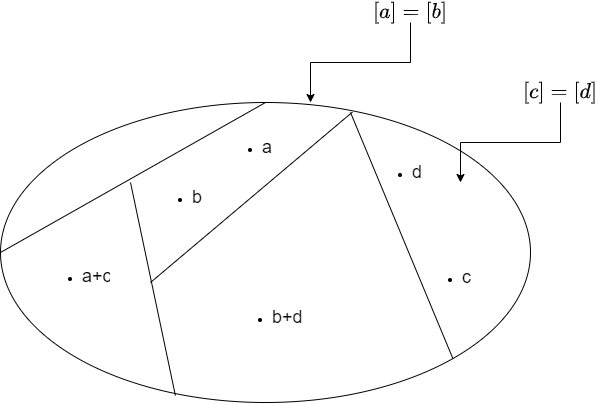
\includegraphics[width=0.6\textwidth]{Figures/partitin_equiv_example.png}
    \caption{Could this happen ($a$ and $b$ are in the same class and $d$ and $c$ are in the same class but $a+c$ and $b+d$ end up in different classes)? We will show this can never happen (i.e. that the operations are well defined).}
    \label{fig:Bad_partition}
\end{figure}

\noindent We must show that if $a$ and $b$ are the same class and $c$ and $d$ are the sample class, then $[a+c]=[b+d]$ \textit{and} $[a\cdot c]=[b\cdot d]$. We show this with the last part of Lemma 1.3.3.
\setcounter{dummy_lemma}{2}
\begin{lemma}[Part 3]
If $a\equiv b\mod n$ and $c\equiv d\mod n$, then $a+c\equiv b+d\mod n$ AND $a\cdot c\equiv b\cdot d \mod n$.\\
\textit{Proof:}
\begin{align}
a\equiv b\mod n \iff n |(a-b)\nonumber\\
c\equiv d\mod n \iff n |(c-d)\nonumber
\end{align}
Then by Observation \#4, $n|a-b+c-d=(a+c)-(b+d)$ (i.e. $n$ divides the linear combination of $a-b$ and $c-d$ so $a+c\equiv b+d\mod n$. Using observation \# 4 again, we can infer the $n|(a-b)c+(c-d)b=ac-bd$ so $ac\equiv bd\mod n \ \ \blacksquare$\\
\end{lemma}

% \textbf{Lemma 1.3.3 (Pt. 3)} If $a\equiv b\mod n$ and $c\equiv d\mod n$, then $a+c\equiv b+d\mod n$ AND $a\cdot c\equiv b\cdot d \mod n$.\\
% \textit{Proof:}
% \begin{align}
% a\equiv b\mod n \iff n |(a-b)\nonumber\\
% c\equiv d\mod n \iff n |(c-d)\nonumber
% \end{align}
% Then by Observation \#4, $n|a-b+c-d=(a+c)-(b+d)$ (i.e. $n$ divides the linear combination of $a-b$ and $c-d$ so $a+c\equiv b+d\mod n$. Using observation \# 4 again, we can infer the $n|(a-b)c+(c-d)b=ac-bd$ so $ac\equiv bd\mod n \ \ \blacksquare$\\
\noindent After having read all three parts of Lemma 1.3.3, one might consider the specific case when $n=2$ again. We see that the "parity", i.e. the odd-ness or even-ness of an integer, exactly corresponds to the two possible equivalence classes for an integer $a\in \Z$ under the relation $\equiv\mod 2$. That is,
\begin{align}
    a\sim0 \iff 2|a-0 \iff 2|a &\iff a \text{ is even} \nonumber \\
    a\sim1 \iff 2|a-1 \iff a-1 \text{ is even} &\iff a \text{ is odd} \nonumber
\end{align}
In this way, we can see that the equivalence relation $\equiv\mod n$ generalizes the notion of "parity" to $n$ remainder classes, rather than just $+1$ or $+0$ remainder classes like congruence $\mod 2$ does. Similarly, Part 3 of this lemma specifically, vastly generalizes the well-established facts that: 
\begin{align}
    \text{even}+\text{even}&=\text{even} &\iff &[0]+[0]=[0] \text{ \ \ and }& \text{even}\cdot \text{even} &=\text{even} &\iff [0]\cdot [0]=[0]\nonumber \\
    \text{even}+\text{odd}&=\text{odd} &\iff &[0]+[1]=[1] \text{ \ \ and }& \text{even}\cdot \text{odd} &=\text{even} &\iff [0]\cdot [1]=[0] \nonumber \\
    \text{odd}+\text{even}&=\text{odd} &\iff &[1]+[0]=[0] \text{ \ \ and }& \text{odd}\cdot \text{even} &=\text{even} &\iff [1]\cdot [0]=[0] \nonumber \\
    \text{odd}+\text{odd}&=\text{even} &\iff &[1]+[1]=[0] \text{ \ \ and }& \text{odd}\cdot \text{odd} &=\text{odd} &\iff [1]\cdot [1]=[1] \nonumber 
\end{align}
Another interesting consequence is that, e.g. in $\Z_{10}=\{[0],[1],...,[9]\}$ if we know the equivalence class of $30057=3005\cdot(10)+7 \implies [30057]=[7]$, and the equivalence class of $402=40\cdot(10)+2 \implies [402]=[2]$ then we can immediately determine the equivalence class of $402\cdot 30057$ without ever even computing the full product, it is simply $[2]\cdot[7]=[2\cdot 7]=[14]=[4]$. Lemma 1.3.3 part 3 says this same trick can be applied when considering arbitrary classes $[0], [1], ... , [n-1]$ under the equivalence relation $\equiv \mod n$. \steezybreak\\
\noindent Ok that's it for congruences, next lecture: Groups! $\smiley{}$
